\subsection{Spike-by-Spike Neural Networks}
\label{sec:sbs}

Technically, SbS is a spiking neural network approach based on a
generative probabilistic model. It iteratively finds an estimate of
its input probability distribution $p(s)$ (i.e. the probability of
input node $s$ to stochastically send a spike) by its latent variables
via $r(s) = \sum_i h(i) W(s|i)$. 
where $\vec{h}$ is an inference
population composed of a group of neurons that compete with each
other. An inference population sees only the spikes $s_t$ (i.e. the
index identifying the input neuron $s$ which generated that spike at
time $t$) produced by its input neurons, not the underlying input
probability distribution $p(s)$ itself. By counting the spikes
arriving at a group of SbS neurons, $p(s)$ is estimated by
$\hat{p}(s) = 1/T \sum_t \delta_{s,s^t}$ after $T$ spikes have been
observed in total. The goal is to generate an internal representation
$r(s)$ from the string of incoming spikes $s_t$ such that the negative
logarithm of the likelihood
$L = C - \sum_\mu \sum_s \hat{p}_\mu(s) log\left( r_\mu(s) \right)$ is
minimized. $C$ is a constant which is independent of the internal
representation $r_\mu(s)$ and $\mu$ denotes one input pattern from an
ensemble of input patterns. Applying a multiplicative gradient descent
method on $L$, an algorithm for iteratively updating $h_\mu(i)$ with
every observed input spike $s_t$ could be derived
\cite{ernst2007efficient}
  \begin{eqnarray} \label{eq:sbs_update}
  h_\mu^{new}(i) = \frac{1}{1+\epsilon} \left(h_\mu(i) + \epsilon \frac{h_\mu(i) W(s_t|i) }{\sum_j h_\mu(j) W(s_t|j)} \right) 
  \end{eqnarray}
  where $\epsilon$ is a parameter that also controls the strength of sparseness of the distribution of latent variables $h_\mu(i)$. Furthermore, $L$ can also be used to derive online and batch learning rules for optimizing the weights $W(s|i)$. The interested reader is referred to \cite{ernst2007efficient} for a more detailed exposition.

  \REVIEW{ From a practical point of view, SbS provides a mechanism to obtain a sparse representation of input patterns. Given a set of
    training samples $\{x_\eta\}$ it learns weights, W, that allow
    to express the input patterns as a linear sparse non-negative combination
    of features.  During inference, it provides a mechanism express
    each the test input $x_\mu$ as $x_\mu \approx W\, h_\mu$ where all
    entries are non-negative.

    The inference procure consist in generating indices $s_t$
    distributed according to a categorical distribution of the input pattern
    $s_t \sim \mathrm{Categorical}(x_{\mu}(0), x_{\mu}(1), ..,
    x_{\mu}(N-1))$. Starting with a random $h$ and executing
    iteratively \mbox{\Equ{eq:sbs_update}} the SbS algorithms finds
    $h_{\mu}$. The fundamental concept of SbS can be extended from vector to matrix
    inputs. In this case, the linear operation $W\, h_\mu$ can be replaced by a
    convolution to obtain a convolutional SbS layer.}

%%%% This is added by Yarib, please review it
%%%%\subsection{Parallelization in SbS networks}
Further on,  SbS network models can be constructed in sequential layered structures \cite{rotermund2019Backpropagation}, where each layer consists of many inference populations (IPs), which can be simulated independently while the communication between the IPs is organized by a low bandwidth signal -- the spikes. Technically, each IP is an independent computational entity (see \fig{fig:SbS_layer}). This allows to design specialized hardware architectures that can be massively parallelized.

\begin{figure}
	\centering
	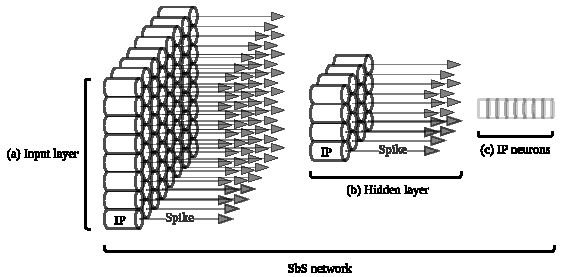
\includegraphics[width=0.5\textwidth]{../figures/SbS_layer.pdf}
	\caption{SbS IPs as independent computational entities, (a) illustrates an input layer with a massive amount of IPs operating as independent computational entities, (b) shows a hidden layer with an arbitrary amount of IPs as independent computational entities, (c) exhibits a set of neurons grouped in an IP. }
	\label{fig:SbS_layer}
\end{figure}


% Fundamentally, SbS is a stochastic gradient descent dynamics
% consistent with Non-Negative Matrix Factorization (NNMF). The stochasticity of gradient descent could
% in principle overcome local minima.  Furthermore, it favors sparse
% solutions with little fluctuations (which is the case for overcomplete
% representations). Finally this specific mechanism for inducing
% sparseness selects those sparse solutions that are robust against
% noise in the inputs.

% In SbS, the expected change at a
% given h-state (i.e. $\Delta h^{s_t}_i 	\propto \left<
% \frac{W(s_t | i) h_i}{\sum_j W(s_t | j) h_j} - 1 \right>_{p(s_t)}$ for all
% $i \in (1,...,N)$ is exactly the same we would have in a low pass
% version of NNMF ($\Delta h_i
% = \sum_s \frac{p(s) W(s | i) h_i}{\sum_j W(s | j) h_j} - 1$). Then,
% for each given h-state, the changes of h induced by SbS consist of the
% expected vector $\Delta h$ plus fluctuations $\eta_i(s_t)$ with
% $<\eta_i(s_t)>p(s_t) = 0$
% (i.e. $\Delta h^{s_t}_i = \sum_s \frac{p(s) W(s | i) h_i}{\sum_j W(s | j) h_j} + \eta_i(s_t)$).
% Thus, SbS performs a random walk with mean $\Delta h$ and some variance, where we have a stochastic process in h-space with the correct
% drift ($\Delta h$) and diffusion. Such processes drift towards states where the drift vanishes except for
% remaining fluctuations. Thus, it produces a Brownian motion
% finally leading to a probability density for h-states centered around
% the fixed point.

% However, even in cases where the problem is convex, NNMF can still have
% manifolds of equivalently optimal solutions. That is, the fixed points
% are not necessarily unique. This is particularly the case for
% overcomplete representations, which can occur when the number of output
% nodes is larger than the number of input nodes. Here, SbS has a tendency
% to select those solutions that have smaller fluctuations of the
% h-values. Simply because h-states with larger fluctuations have a
% smaller probability density in stochastic processes. In the overcomplete
% case these h-vectors are sparse.

% But not only sparseness is favored by SbS, but additionally those among
% the sparse solutions that have the smallest fluctuations. This is the
% famous tornado in the example in the 2008 paper.

\begin{figure}
  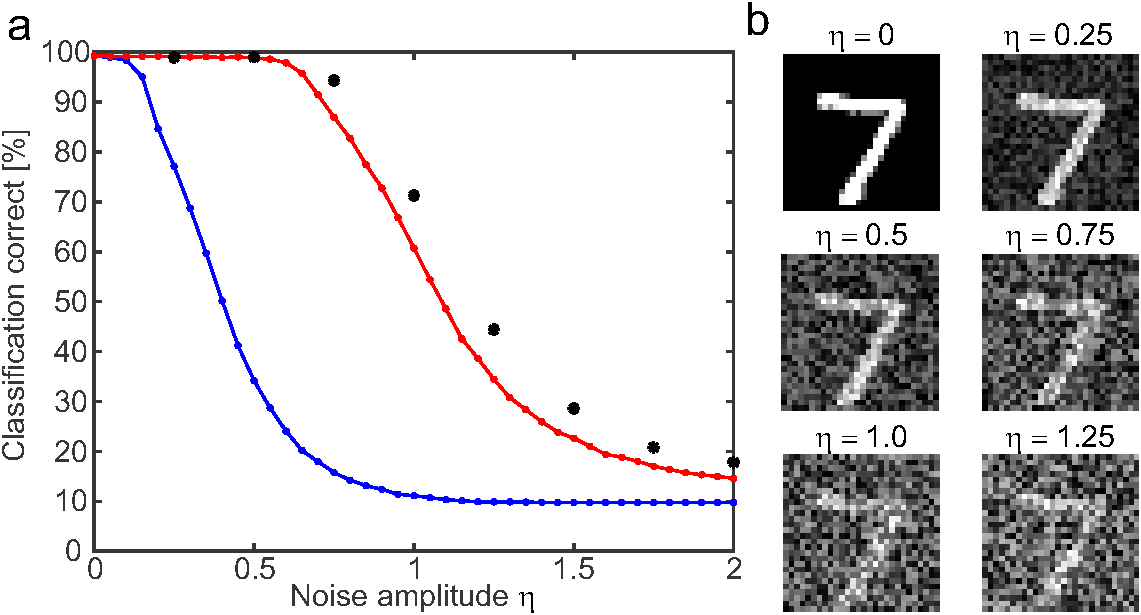
\includegraphics[width=\columnwidth]{../figures/sbs_robustnes.pdf}
  \caption{(a) Performance classification of SbS NN versus equivalent CNN, and (b) example of the first pattern in the MNIST test data set with different amounts of noise.}
  \label{fig:robustnes_sbs}
\end{figure}

To illustrate the advantages of SbS, an example of the noise tolerance of SbS is presented in
\fig{fig:robustnes_sbs}. It compares the classification performance of
a SbS network and a standard convolutional network, with the same amount of
neurons per layer as well as the same layer structure. We trained on MNIST dataset\cite{lecun1998mnist} without noise (see \cite{rotermund2019Backpropagation} for details). The figure shows the correctness for the MNIST test set with its $10000$ patterns in dependency of the noise level for positive additive
uniformly distributed noise. The blue curve shows the performance for
the tensor flow network, while the red curve shows the performance for
the SbS network with 1200 spikes per inference population. Beginning
with a noise level of 0.1, the respective performances are different
with a p - level of at least $10^{-6}$ (tested with the Fisher exact
test). Increasing the number of spikes per SbS population to 6000
(performance values shown as black stars), shows that more spike can
improve the performance under noise even more.

